\SetKwProg{Proc}{procedure}{}{}
\SetKwFunction{Search}{SEARCH}
\SetKwFunction{SampleParticle}{SAMPLE-PARTICLE}
\SetKwFunction{Simulate}{SIMULATE}
\SetKwFunction{Timeout}{TIMEOUT}
\SetKwFunction{Maxstep}{MAX-STEP}
\SetKwFunction{SearchBest}{SEARCH-BEST}
\SetKwFunction{UCB}{UCB}
\SetKwFunction{Rollout}{ROLLOUT}
\SetKwFunction{UpdateBelief}{UPDATE-BELIEF}
\SetKwFunction{ComputeConfidence}{CONF}
\SetKwFunction{SelectBestHypothesis}{SELECT-FACT}
\SetKwFunction{QuerySource}{QUERY}
\SetKwFunction{FilterBelief}{FILTER}

\section{Method}~\label{method:method}
To determine when and what to query the user, we maintain a particle-based belief state to quantify uncertainty and identify task-relevant information. However, particle sampling in large state spaces is computationally expensive, and unconstrained sampling may produce states that violate symbolic constraints. To address these challenges, we propose a frontier-based particle sampling approach that uses symbolic action models to maintain a constraint-consistent belief for query selection.

\subsection{Planning and Querying}~\label{method:overview}\label{method:planning}\label{method:PM}
We maintain a knowledge state $s_t^{K}$ for symbolic planning and execution. For online action selection, we employ POMCP~\cite{silver2010monte}, restricting tree expansion and rollout to symbolically applicable actions. At each step, the planner selects an action $a_t\in\mathcal{A}$ applicable to $s_t^{K}$, denoted by $a_t\llbracket s_t^{K}\rrbracket$. Following execution and observation $o_{t+1}$, we construct a weighted belief $\mathcal{B}_{t+1}$ by sampling from the reachable-state frontier defined by $(s_t^{K},a_t)$. This restricts belief construction to symbolically valid successors while capturing uncertainty in the action outcome.

\subsubsection{When to Query}~\label{method:when}
To determine when to query, we assess uncertainty about the current state through the entropy of the weighted belief. If several successor states remain plausible after an action and no single state is dominant, the robot cannot confidently identify its current state. In this situation, belief entropy is high because the weight is distributed across several possible states. We use this property of entropy to compute confidence from normalized belief entropy~\cite{qu2023stochastic}, where lower confidence indicates greater state uncertainty.

We observe that a symbolic action usually changes only part of the state. Based on this observation, we define the \textit{frontier} of reachable successor states as follows.
\begin{equation}
\mathcal{F}_{t+1}
=
\mathrm{Frontier}(s_t^{K},a_t)
=
\{s_{t+1}^{1},\ldots,s_{t+1}^{j}\}.
\label{eq:frontier}
\end{equation}
For example, an action to pick a tomato can change which object the robot holds but preserves the robot location. Uncertain outcomes within the frontier are mutually exclusive, and no two successor states are identical. We restrict particle sampling to this frontier instead of the entire symbolic state space.

We construct the weighted belief by assigning a normalized weight $w_k$ to each of the $j$ sampled frontier states $s_{t+1}^{k}$.

\begin{equation}
\mathcal{B}_{t+1}
=
\{(s_{t+1}^{k},w_k)\}_{k=1}^{j},
\qquad
\sum_{k=1}^{j}w_k=1.
\label{eq:symbolic_belief}
\end{equation}
We compute these weights by normalizing the product of the transition probability and observation likelihood for each state.
\begin{equation}
\begin{aligned}
\bar{w}_{k}
&=T(s_{t+1}^{k}\mid s_t^{K},a_t)\,
O(o_{t+1}\mid s_{t+1}^{k},a_t),\\
w_k&=\frac{\bar{w}_k}{\sum_{\ell=1}^{j}\bar{w}_{\ell}}.
\end{aligned}
\label{eq:belief_update}
\end{equation}
If all $\bar{w}_k$ are zero, we set $w_k=1/j$.

This explicit weighted frontier is used for confidence estimation and query selection. POMCP maintains sampled states in the search tree to estimate action values. Both components use the same symbolic transition and observation models.

We compute the entropy of the belief as
\[
\mathcal{H}(\mathcal{B}_{t+1})
=
-\sum_{k=1}^{j}w_k\log_2 w_k.
\]
Because the maximum entropy depends on the number of represented worlds, we normalize by $\log_2 j$ and define
\begin{equation}
\mathrm{Conf}(\mathcal{B}_{t+1})
=
1-\frac{\mathcal{H}(\mathcal{B}_{t+1})}{\log_2 j}.
\label{eq:compute_confidence}
\end{equation}
For $j=1$, we define $\mathrm{Conf}(\mathcal{B}_{t+1})=1$. The score approaches zero if the represented states have similar weights and approaches one if most of the belief weight lies on one state.

Given a predefined threshold $\tau\in[0,1]$, the robot initiates state verification if
\begin{equation}
\mathrm{Conf}(\mathcal{B}_{t+1})<\tau.
\label{eq:when_query}
\end{equation}
A higher threshold $\tau$ requires a more concentrated belief and can increase the number of verification queries.

\begin{figure}[t]
\captionsetup{skip=0pt}
\centering
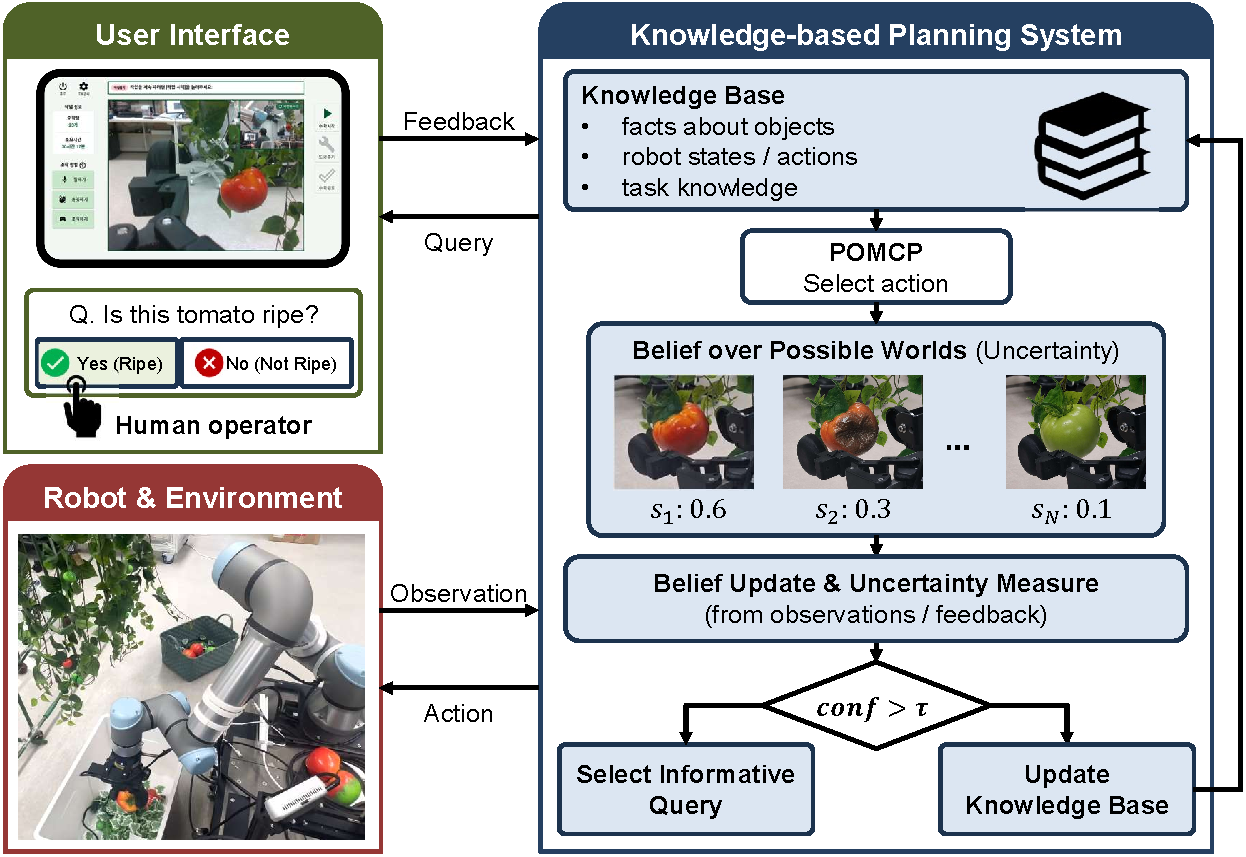
\includegraphics[width=0.98\linewidth]{figures/fig_overview.pdf}
\caption{Online planning with belief-guided state verification. After executing an action and receiving an observation, the planner constructs a weighted belief over reachable symbolic states. Belief confidence determines whether to enter the query loop, and expected entropy reduction determines which symbolic fact to verify. The most probable remaining state becomes the symbolic reference for the next planning step.}
\label{fig:pm}
\end{figure}

\subsubsection{What to Query}~\label{method:what}
If belief confidence falls below $\tau$, the robot triggers a query and must decide which fact to verify. Since verification eliminates state hypotheses that are inconsistent with the answer, we select the fact with the largest expected reduction in belief entropy.

Specifically, we define the query candidate set $\mathcal{Q}(\mathcal{B})$ by extracting atomic facts whose truth values differ across the remaining frontier states in the belief.
\[
\mathcal{Q}(\mathcal{B})
=
\bigcup_{(s,w)\in\mathcal{B}}s
\setminus
\bigcap_{(s,w)\in\mathcal{B}}s.
\]
For each candidate fact $q\in\mathcal{Q}(\mathcal{B})$, we partition the belief according to whether $q$ holds in each state.
\[
\begin{aligned}
\mathcal{B}^{q+}&=\{(s^k,w_k)\mid q\in s^k\},\\
\mathcal{B}^{q-}&=\{(s^k,w_k)\mid q\notin s^k\}.
\end{aligned}
\]
Let $P(q)=\sum_{k:q\in s^k}w_k$ and $P(\neg q)=1-P(q)$. Entropy within each subset is computed after conditionally normalizing its weights. The expected posterior entropy of asking about $q$ is
\[
\mathbb{E}[\mathcal{H}\mid q]
=
P(q)\mathcal{H}(\mathcal{B}^{q+})
+
P(\neg q)\mathcal{H}(\mathcal{B}^{q-}).
\]
The selected query is
\begin{equation}
q^*
=
\arg\min_{q\in\mathcal{Q}(\mathcal{B})}
\left[
P(q)\mathcal{H}(\mathcal{B}^{q+})
+
P(\neg q)\mathcal{H}(\mathcal{B}^{q-})
\right].
\label{eq:select_hypo}
\end{equation}
Eq.~\ref{eq:select_hypo} selects the fact $q^*$ that maximizes expected entropy reduction. The robot then converts this fact into a binary query about the current state. For example, $q^*=\texttt{ripe}(\text{tomato}_1)$ produces the question \textit{`Is tomato 1 ripe?'}. Based on the response $y\in\{\texttt{true},\texttt{false}\}$, the robot updates the belief by removing states inconsistent with the reported truth value.
\begin{equation}
\mathcal{B}
\leftarrow
\begin{cases}
\{(s^k,w_k)\mid q^*\in s^k\}, & y=\texttt{true},\\
\{(s^k,w_k)\mid q^*\notin s^k\}, & y=\texttt{false}.
\end{cases}
\label{eq:filter}
\end{equation}
The retained weights are renormalized, confidence is recomputed, and another fact is selected if confidence remains below $\tau$. The loop ends if the threshold is met or no differentiating fact remains. The robot then commits the maximum a posteriori state
\[
s_{t+1}^{K}
=
\arg\max_{s^k\in\mathcal{B}_{t+1}}w_k
\]
for subsequent symbolic planning.

Alg.~\ref{alg:online_planning} explains the overall online planning and querying procedure. The robot first initializes the belief, step counter, and action sequence (line~\ref{alg1_planning:initialize}). At each step, POMCP selects an action (line~\ref{alg1_planning:search}), and execution stops if no action is available (line~\ref{alg1_planning:dead_end}). Otherwise, the robot executes the action  (lines~\ref{alg1_planning:execute} and~\ref{alg1_planning:record}), then constructs the weighted frontier belief and computes confidence (lines~\ref{alg1_planning:belief_update} and~\ref{alg1_planning:compute_conf}). If confidence falls below $\tau$, the robot selects a candidate fact (line~\ref{alg1_planning:select_hypo}). If no candidate remains, the query loop ends (line~\ref{alg1_planning:no_candidate}). Otherwise, the robot obtains an external response and filters the belief (lines~\ref{alg1_planning:query} and~\ref{alg1_planning:filter}), then recomputes confidence (line~\ref{alg1_planning:recompute_conf}). After the query loop, the most probable remaining state becomes the next symbolic planning state (line~\ref{alg1_planning:commit}). Appx.~\ref{appx:algorithms} provides the detailed POMCP search, simulation, and rollout procedures.

\begin{algorithm}[t]
\caption{Belief-Guided State Verification and Planning}
\label{alg:online_planning}
\DontPrintSemicolon
\textbf{Input}\quad initial state $s_0^{K}$, confidence threshold $\tau$, step limit $T_{\max}$\;
\textbf{Output}\quad executed action sequence $\pi$\;
\BlankLine
$\mathcal{B}\gets\{(s_0^{K},1)\}\qquad t\gets0\qquad \pi\gets()$\label{alg1_planning:initialize}\;
\While{$t<T_{\max}$}{
    $a_t\gets$\Search{$\mathcal{B}$}\label{alg1_planning:search}\;
    \If{$a_t=\emptyset$}{
        \textbf{break}\label{alg1_planning:dead_end}\tcp*{dead end}
    }
    execute $a_t$ and receive $o_{t+1}$\label{alg1_planning:execute}\;
    $\pi\gets\pi\mathbin{\|}a_t$\label{alg1_planning:record}\;
    $\mathcal{B}\gets$\UpdateBelief{$s_t^{K},a_t,o_{t+1}$}\label{alg1_planning:belief_update}\;
    $c\gets\mathrm{Conf}(\mathcal{B})$\label{alg1_planning:compute_conf}\;
    \While{$c<\tau$}{
        $q^*\gets$\SelectBestHypothesis{$\mathcal{B}$}\label{alg1_planning:select_hypo}\;
        \If{$q^*=\emptyset$}{
            \textbf{break}\label{alg1_planning:no_candidate}\tcp*{no differentiating fact}
        }
        $y\gets$\QuerySource{$q^*$}\label{alg1_planning:query}\;
        $\mathcal{B}\gets$\FilterBelief{$\mathcal{B},q^*,y$}\label{alg1_planning:filter}\;
        $c\gets\mathrm{Conf}(\mathcal{B})$\label{alg1_planning:recompute_conf}\;
    }
    $s_{t+1}^{K}\gets\arg\max_{s^k\in\mathcal{B}}w_k$\label{alg1_planning:commit}\;
    $t\gets t+1$\label{alg1_planning:advance}\;
}
\KwRet $\pi$\label{alg1_planning:return}\;
\end{algorithm}

\subsection{System Implementation}~\label{method:modules}
\begin{figure*}[t!]
\captionsetup{skip=0pt}
\centering
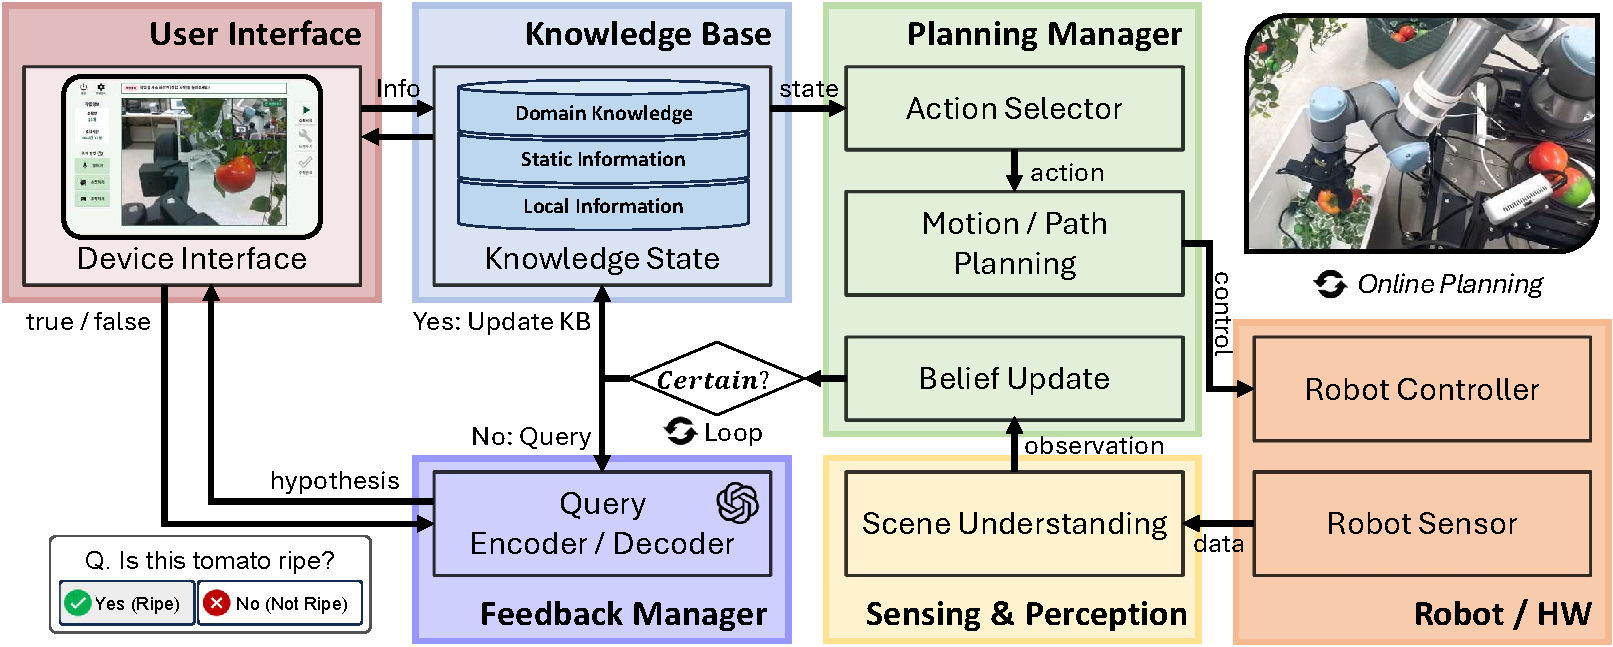
\includegraphics[width=0.95\linewidth]{figures/fig_dataflow.pdf}
\caption{Framework for robot execution of the proposed planning and querying method.}
\label{fig:data_flow}
\end{figure*}

We implement a modular framework to execute the proposed planning and querying method on a robot, as shown in Fig.~\ref{fig:data_flow}. The Knowledge Base (KB) stores symbolic facts and action models, and Sensing and Perception (SP) provides observations and numeric state estimates from sensor data. The Planning Manager (PM) uses this information to select robot actions, construct the frontier belief, and decide when and what to query. The Feedback Manager (FM) converts the selected fact into a question and the response into evidence for the belief update. The User Interface (UI) presents the questions and collects responses during human interaction.

\label{method:KB}
The KB partitions information into domain knowledge $\mathcal{I}^{D}$, static structured information $\mathcal{I}^{S}$, and local information $\mathcal{I}^{L}$ obtained during execution.
\[
\mathcal{KB}=\mathcal{I}^{D}\sqcup\mathcal{I}^{S}\sqcup\mathcal{I}^{L}.
\]
Domain knowledge contains action schemas and task rules. Static information includes invariant facts and fixed map or robot parameters. Local information contains perceptual facts and numeric fluents that are updated during execution. SP maps raw sensor input to these task-level observations. For example, RGB-D sensing can update object pose and ripeness estimates, while the symbolic observation likelihood determines how those observations weight the frontier states.

\label{method:action_execution}
Each symbolic action invokes a robot skill. Actions such as $\texttt{navigate}(\text{robot},l_1,l_2)$ and $\texttt{pick}(\text{robot},\text{tomato}_1)$ specify task-level intentions, while an off-the-shelf motion planner such as MoveIt~\cite{chitta2012moveit} uses numeric fluents from the KB to generate low-level motion. This separation allows the feedback policy to operate on task-level facts without depending on a particular motion-planning implementation.

\label{method:FM}
The FM maps the selected predicate to a predefined question template and converts the response to a Boolean value. During human interaction, the tablet UI displays the camera view, highlights the referenced object with a bounding box, and presents simple response options. Participants answer questions about the displayed state fact, and the planner selects the next robot action.
